\section{LSRs and \textit{MPLS clusters}}\label{cluster}
% %%%%%%%%%%%%%%%%%%%%%%%%%%%%%%%%%%%%%%
To the best of our acknowledge, MPLS interconnection architecture on Internet
topology has not yet been studied. In this way, we focus our attention on
studying several LSRs properties and \dfn{MPLS clusters} (i.e., set of MPLS
graphs) and their interactions with non MPLS networks. Our study aims at better
understanding the impact of MPLS deployments over Internet, specifically over
router level topology.

\subsection{Definitions and Background}\label{cluster.methodo}
% %%%%%%%%%%%%%%%%%%%%%%%%%%%%%%%%%%%%%%
\begin{figure*}[!htb]
  \begin{center}
    \subfigure[Degree Distribution Probability]{\label{fig_degree_distribution}
      \includegraphics[width=5.5cm]{DegreeDistribution}}\hfil
    \subfigure[Clustering Coefficient]{\label{fig_clustering}
      \includegraphics[width=5.5cm]{ClusteringCoeficient}}\hfil
    \subfigure[Neighbor Degree Distribution]{\label{fig_neighbor}
      \includegraphics[width=5.5cm]{NearestNeighbor}}
  \end{center}
\caption{Metrics for IP, router and MPLS cluster interconnection
topologies.} 
\label{fig_metrics}
\end{figure*}

\begin{table}[!t]
  \begin{center}
    \begin{tabular}{l|ll}
    \textbf{Graph} & \textbf{Notation} & \textbf{Definition}\\
    \hline
    IP                 & $G_{ip}$ & $(V_{ip}, E_{ip})$\\
    Router             & $G_r$ & $(V_r, E_r)$\\    
    MPLS               & $G_r^{mpls}$ & $(V_r^{mpls}, E_r^{mpls})$\\
    ASes induced graph & $G_r(as)$ & $(V_r(as), E_r(as))$\\    
    MPLS cluster       & $C_i^{mpls}$ & /\\
    MPLS cluster interconnection graph & $G_{r \backslash lsr}$ & $(V_{r
    \backslash lsr}, E_{r \backslash lsr}^{mpls})$
    \end{tabular}
  \end{center}
  \caption{Summary of graph notations used in Sec.~\ref{cluster}.}
  \label{cluster.table_notations}
\end{table}

We defined several graphs at different abstraction levels as follows (they are
summarized in Table~\ref{cluster.table_notations}): The \dfn{IP level graph} is
defined as $G_{ip}=(V_{ip}, E_{ip})$, where $V_{ip}$ is the IP addresses
discovered in our exploration and $E_{ip}$ the set of the links found trough
\traceroute.   Second, the \dfn{router level graph} is defined as $G_{r}=(V_{r},
E_{r})$, where $V_{r}$ is the set of routers (alias resolution having been done
through MIDAR~\cite{Keys13}), and $E_{r}$ is the set of all the links found
between any pair of routers $v \in V_{r}$. Third, the \dfn{MPLS router level
graph} refers to $G^{mpls}_{r}=(V^{mpls}_{r}, E^{mpls}_{r})$ where
$V^{mpls}_{r}$ is the set of routers in which at least one IP interface belongs
to an LSP, and  $E^{mpls}_{r}$ is the set of all \textit{mpls links}
$(v^{mpls}_{r}(i), v^{mpls}_{r}(j))$ such as
$\{{v^{mpls}_{r}(i)},{v^{mpls}_{r}(j)} \}\in V^{mpls}_{r}$.

The \dfn{ASes induced graph} is defined as $G_{r}(as)=(V_{r}(as), E_{r}(as))$.
Each vertex in $G_{r}(as)$ has an interface belonging to the same Autonomous
System, $as$.  In particular, the induced graph of $G_r^{mpls}$ is
$G^{mpls}_{r}(as)=(V^{mpls}_{r}(as), E^{mpls}_{r}(as))$.  This definition allows
us to define an \dfn{MPLS cluster}, $C^{mpls}_{i}$, as a connected component $i$
of $G^{mpls}_{r}(as)$. A given AS may have several MPLS clusters.

Finally, the \dfn{MPLS cluster interconnection graph} is an hybrid router level
graph,  $G_{r\backslash lsr}=(V_{r\backslash lsr},E^{mpls}_{r\backslash lsr})$,
where all the MPLS clusters $C^{mpls}_{i}$ are gathered together in a single
node $v\in V_{r\setminus ls}$, while non-MPLS capable routers remain unchanged.
Broadly speaking, an MPLS cluster interconnection graph refers to a router level
graph where all MPLS clusters are treated as a single node. In this way, we can
study how IP interfaces and non MPLS capable routers interact with MPLS
clusters. Additionally, we call $G_{r\backslash lsr}(as)$ to the induced
subgraphs of $G_{r\backslash lsr}$ by routers having at least one interface in
the Autonomous System $as$.

% \textbf{IP level Graph:} $G_{ip}=(V_{ip}, E_{ip})$, where $V_{ip}$ is the IP
% address discovered in our exploration and $E_{ip}$ is the set of the links found
% trough traceroute. Note that \traceroute just records incident IP addresses in
% a path.

As the analysis is mainly based on $k$-core decomposition, we present the
following definitions:
\begin{itemize}
  \item\dfn{\textit{k}-core:}. Given a graph $G=(V,E)$, then the
  subgraph $H=(C,E|C)$ induced by the set $ C\subseteq V$ is a \textit{k}-core
  of order $k$ $iff$ $\forall v \in C: degree_{H}(v)\geq k$ and $H$ is the
  maximum subgraph with this property.
%A \textit{k}-core of $G$ can therefore be obtained by recursively removing all
% the vertices of degree less than $k$, until all vertices in the remaining
% graph have at least degree $k$.    
  \item\dfn{Shell index}. A vertex $i$ has a shell index $c$ if it
  belongs to the $c$-core but not to $(c+1)$-core. We denote by $C_i$ the shell
  index of vertex $i$. A shell $C_c$ consists of all the vertices whose shell
  index is $c$. The maximum value $c$ such that $C_c$ is not empty is denoted by
  $C_{\max}$.  Therefore, the $k$-core is thus the union of all shells $C_c$ with
  $c \geq k$.
\end{itemize}

To retrieve the $k$-core decomposition of a graph $G$, we use
\lanet\cite{Alvarez06k}.  This tool returns a two dimensional plot,
where the position of each vertex depends on its shell index and its neighbors'
index. A color code allows for the identification of shell indices, while the
vertex's original degree is provided by its size \ed{size of what?  circles on
Fig.~\ref{fig_k_core_MPLS} for instance?}, which depends logarithmically on the
degree. A central role in the visualization method is played by multi-components
representation of $k$-cores.  \ed{It is unclear to me what's a multi-component
representation.  The next sentences in this paragraph are also unclear} In the
most general situation, the recursive removal of vertices having degree less
than a given $k$ can break the original network into various connected
components, each of which might even be once again broken by the subsequent
decomposition.

In this paper, we use $k$-core decomposition focused on properties around mpls
clusters interconnection.  \lanet is useful to read basic features of the graph
(degree, hierarchical structure, etc.) as well as more entangled features, e.g.,
the relation between a vertex and the hierarchical position of its neighbors. It
is also useful to  discriminate between networks with different topological
properties and structural arrangement. This provides us an idea about the
structural arrangement and topological properties caused by MPLS usage.
Additionally, the visualization helps us to find properties and fingerprints
tightly related with MPLS presence.

\subsection{MPLS on Internet Topology}\label{cluster.topo}
% %%%%%%%%%%%%%%%%%%%%%%%%%%%%%%%%%%%%%%
\begin{figure}[!t]
  \begin{center}
    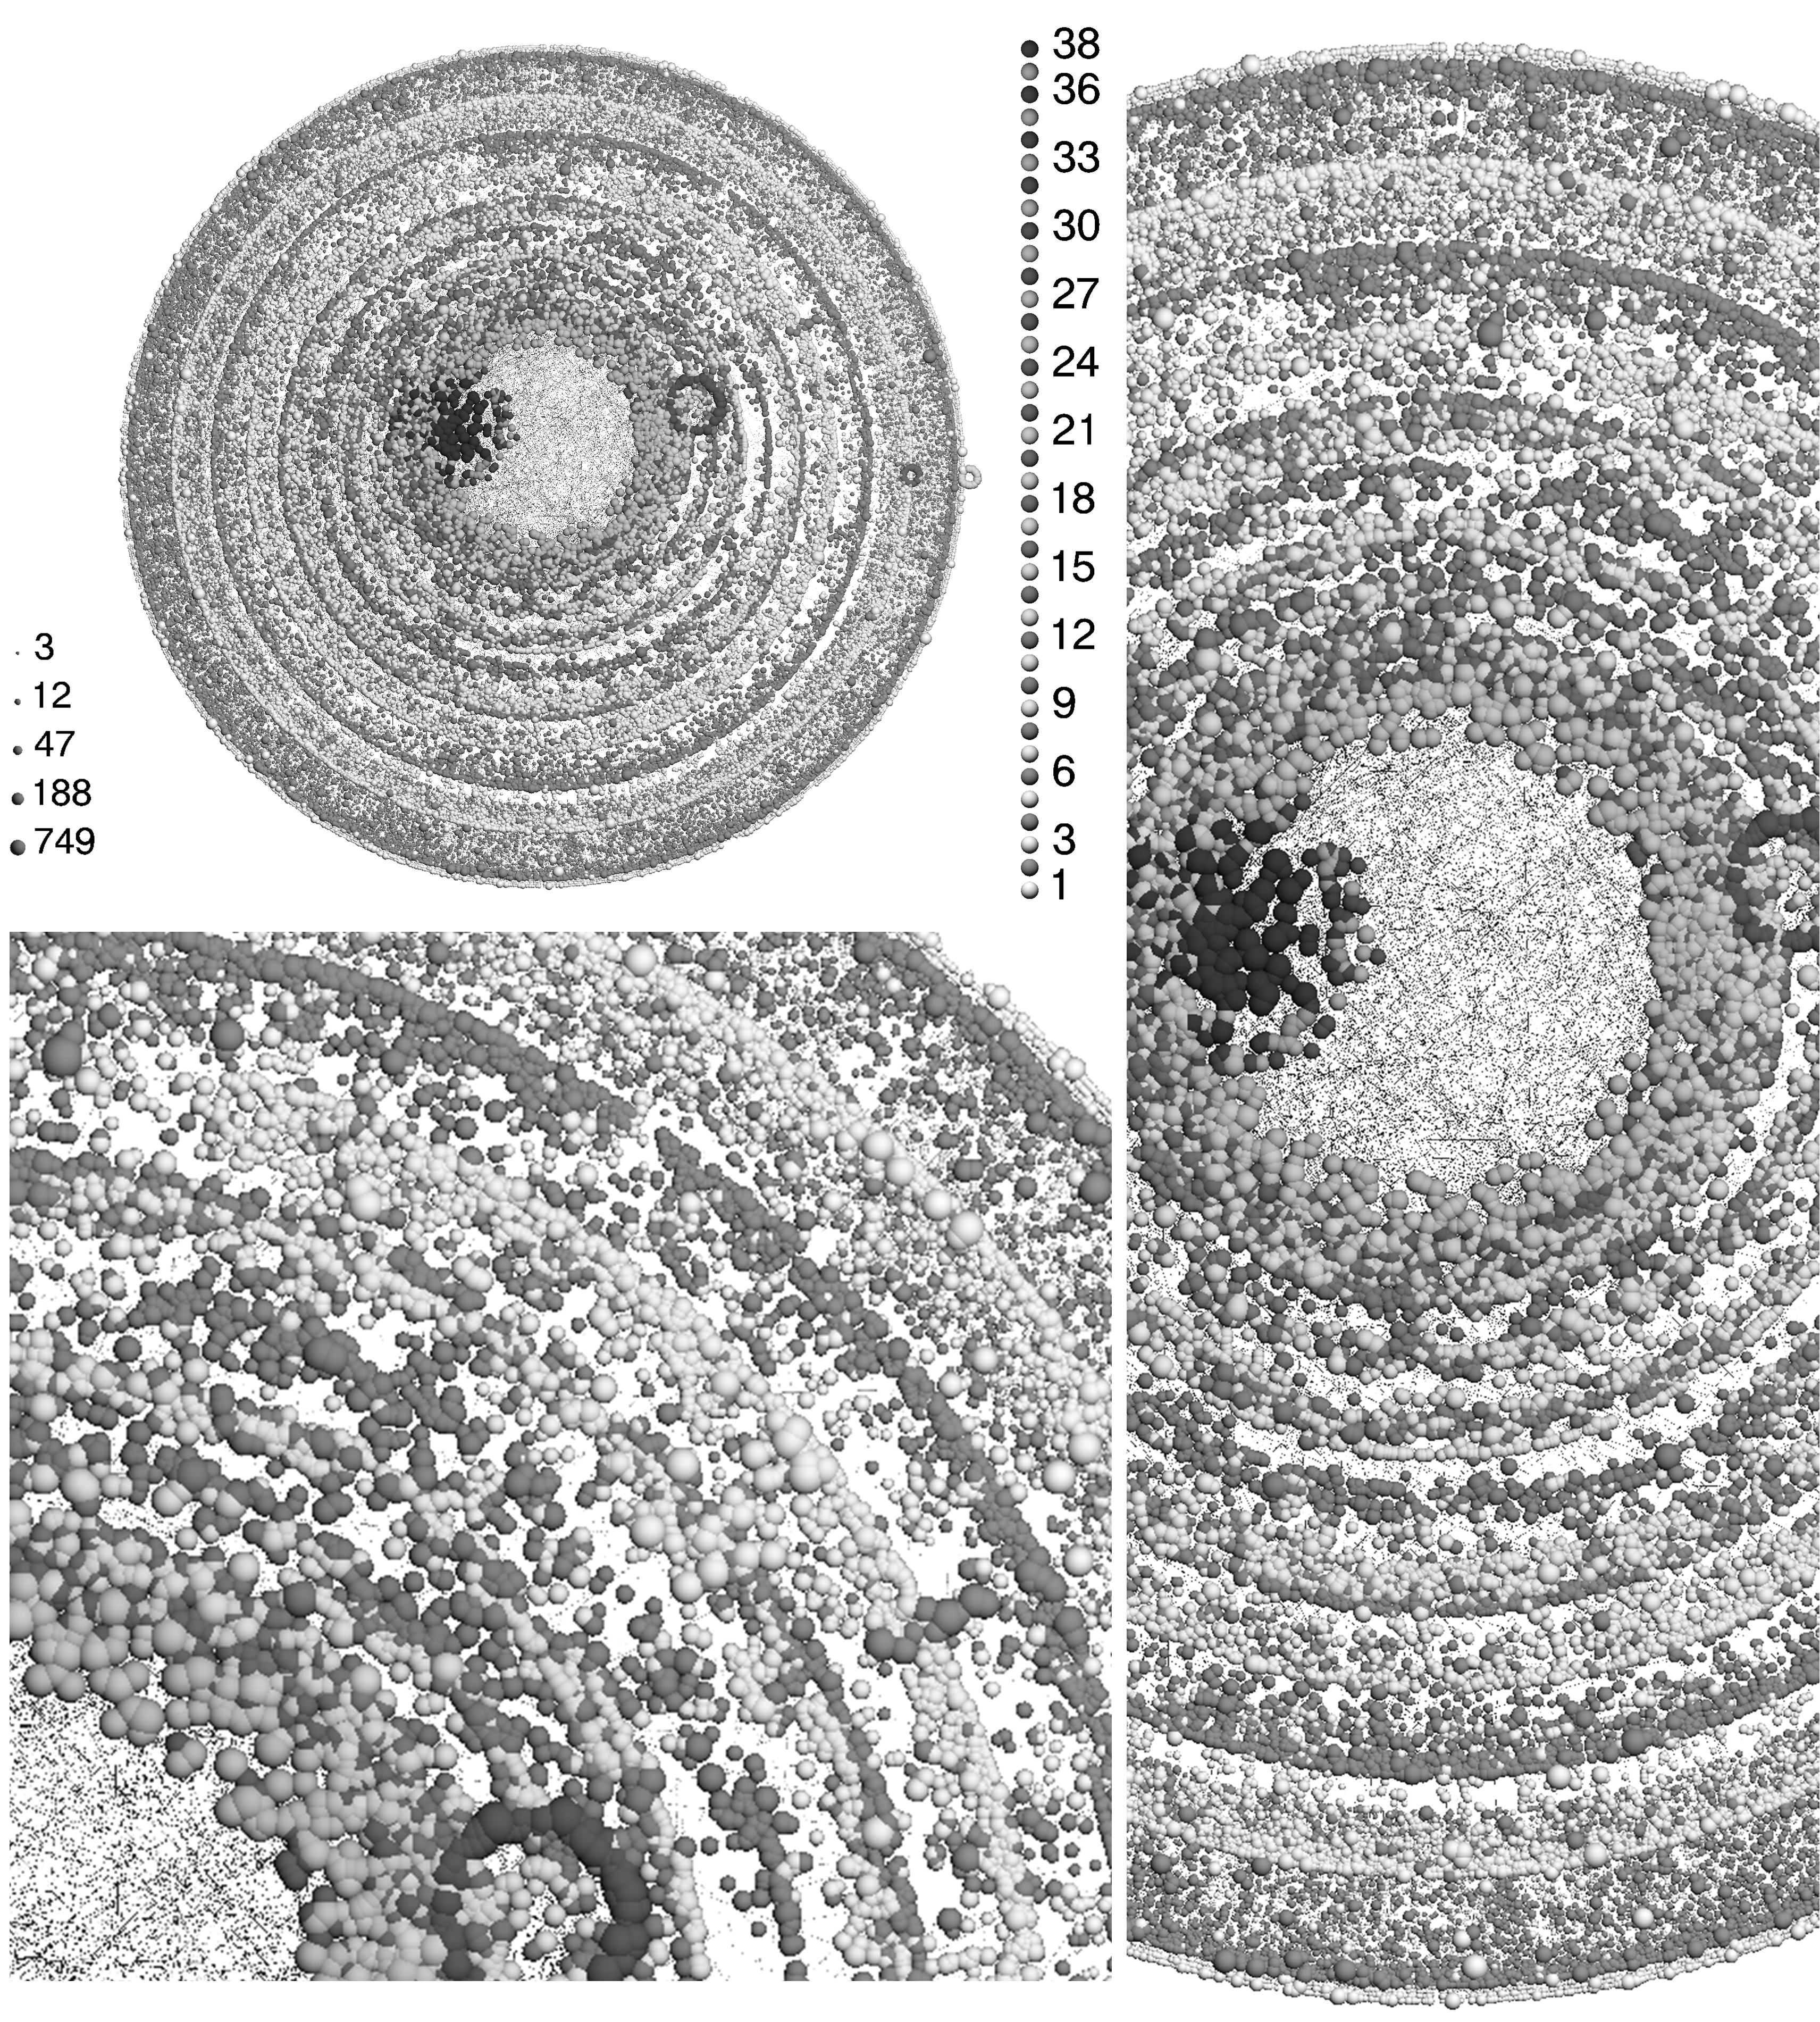
\includegraphics[width=3in]{Routers}
  \end{center}
  \caption{$k$-core visualization of router level topology $G_{r}$.}
  \label{fig_k_core_routers}
\end{figure}

We first analyze the graphs $G_{ip}$ and $G_{r}$ in order to know if there are
some strong differences between their structure and properties. As expected, we
notice that the router level topology has slightly stronger clustering
coefficient than the IP level topology (see Fig.~\ref{fig_clustering}), due to
% the join of IP interfaces into single routers.
alias resolution process.  However, the main structure of both topologies iss
similar as displayed on Fig.~\ref{fig_degree_distribution}
and~\ref{fig_neighbor}. Because we do not see any meaningful difference
between these topologies, and the router level topology is closer to a
realistic Internet one, we use the later for the remaining of our analysis.

Fig.~\ref{fig_k_core_routers} shows the $k$-core visualization of $G_{r}$.  The
figure is divided in three parts, the main part being in the upper left while
the two others are a zoom on the main part.  The main part is composed of two
scales, the one on the left is the node degree scale representing the degree in
a logarithmic scale, while the one on the right is a gray scale with each shell
index $c_i$.  Between the two scales, we see the shell index with $C_{\max}$ in
the center, the other shells being located concentrically around it. Note that
$C_{\max}$-core is made of several components with one having the most
significant part, and it is shown at the left of the center (black nodes).  We
also see that all the shells index are highly populated and that the node degree
is not related with the shell index, i.e., there are many routers with high
degree in the outer (lower) shells.  Another typical feature of router level
topology is that the links between routers mainly occurs between routers
belonging to neighbors shells, e.g., the routers on the outer shells are not
usually connected to the routers located on the  $C_{\max}$-core, as it is in
the Autonomous Systems maps~\cite{Alvarez06k}.

\begin{figure*}[!t]
  \begin{center}
    \subfigure[The $k$-core visualization of router level topology $G_{r}$.]{\label{fig_k_core_LSR}
      \includegraphics[width=18cm]{LSR}}
\hfil
    \subfigure[The $k$-core visualization of MPLS cluster level topology  $G_{r\backslash lsr}$.]{\label{fig_k_core_MPLS}
      \includegraphics[width=18cm]{MPLS}}
  \end{center}
  \caption{$k$-core visualization of $G_r$ and $G_{r \backslash lsr}$.  On
  Fig.~\ref{fig_k_core_LSR}, black nodes refer to non MPLS capable routers and
  gray nodes refer to LSRs.  On Fig.~\ref{fig_k_core_MPLS}, black nodes refer to
  non MPLS capable routers and gray nodes refer to MPLS clusters.} 
  \label{fig_kcore_overview}
\end{figure*}

In order to locate LSRs-routers with MPLS capabilities into the shells index
over $k$-core decomposition, we paint in black the non-MPLS routers and in gray
the LSRs. The results are showed in Fig.~\ref{fig_k_core_LSR}.  For the sake of
the visualization, we do not include neither the shell index, degree scale, nor
edges between shells. We notice that the LSRs are commonly distributed around
the different shells of Internet but slightly tends to concentrate with more
density nearby the $C_{\max}$-core. Additionally, we apply the same methodology
for the MPLS interconnection cluster level graph $G_{r\backslash lsr}$
(Fig.~\ref{fig_k_core_MPLS}): MPLS clusters (gray nodes) are distinguished from
the non MPLS capable routers (black nodes). In this case,  MPLS clusters  are
also spread out on the Internet.  Indeed, we see some well defined gray nodes on
the periphery of the decomposition. However MPLS clusters show a stronger
tendency to concentrate near the $C_{\max}$-core.

Finally, we evaluate the impact of MPLS clusters on the typical router level
topology, i.e., MPLS cluster interconnection graph $G_{r \backslash lsr }$. We
use metrics such as degree distribution, clustering coefficient, and nearest
neighbor degree, as is shown on Fig.~\ref{fig_metrics}.
We notice that MPLS clusters highly impact over the router level topology. On
one hand, the nearest neighbor degree highly increments for low degrees nodes on
$G_{r \backslash lsr }$, suggesting that routers with low degree are highly
connected to MPLS clusters and thereby to LSRs. On the other hand, the
clustering coefficient of $G_{r \backslash lsr }$ change significantly their
slope in regards with IP and router level topology, indicating that routers with
high degree are connected to \textit{common} MPLS clusters. \ed{does this
suggest that some MPLS clusters are more ``popular'' than others?}

\subsection{\textit{MPLS clusters} on Autonomous Systems}\label{cluster.as}
% %%%%%%%%%%%%%%%%%%%%%%%%%%%%%%%%%%%%%%%%%%%%%%%%%%%%%%%%%
Although, the previous results give us a general overview about MPLS deployment,
we believe that the study of MPLS structure requires to go deeper into the
individual AS topology. Indeed, we found that around $89.9\%$ of \textit{mpls
links} are intra-domain. Thereby, we focus on the top ASes in terms of total
number of discovered links.  On this set of ASes, we discard those having less
than 500 mpls links. Additionally, we identify the amount of mpls
links by AS, distinguishing the type of tunnel \ed{unclear}:

\begin{itemize}
  \item[i] \textit{explicit mpls link:} Link between an interface
  $i^{\text{explicitMPLS}}_{n}$  and its immediate previous interface
  $i^{\text{MPLS}}_{n-1}$ discovered by traceroute, such that
  $i^{\text{explicitMPLS}}_{n}$ belongs to an explicit MPLS tunnel and
  $i^{\text{MPLS}}_{n-1}$ belongs to any kind of MPLS tunnel (explicit,
  \textit{qTTL} based or \textit{u-turn} based).
  \item[ii] \textit{qTTL mpls link:} Link between the interfaces
  $i^{\text{qTTL}}_{n}$  and $i^{\text{MPLS}}_{n-1}$, such that
  $i^{\text{qTTL}}_{n}$ belongs to a tunnel \textit{qTTL} based.
  \item[iii] \textit{u-turn mpls link:} Link between the interfaces
  $i^{\text{u-turn}}_{n}$  and $i^{\text{MPLS}}_{n-1}$, such that
  $i^{\text{u-turn}}_{n}$ belongs to a tunnel \textit{u-turn} based.
\end{itemize}

The summary of the top ASes is showed in the Fig.~\ref{top_as}.
We noticed that the ratio $r_{mpls}= \vert E^{mpls}_{r} (as) \vert /\vert E_{r}
(as) \vert $  is greater when more  \textit{explicit mpls links} have been
discovered. Interestingly, we also see that the ASes with more links discovered
have the lowest ratio $r_{mpls}$.

For our purposes, we select the most representatives ASes from those in
Fig.~\ref{top_as}. In this way we analyzed the graphs $G_{r}(as)$ and
$G_{r\backslash lsr}(as)$ for AS1299, AS174, AS6762, AS7018, AS1273 and AS2914.
The most remarkable observation (see Fig.~\ref{fig_cluster_mpls}) occurs
regarding the graph $G_{r\backslash lsr}(as)$: $k$-core decomposition highly
differs on those ASes, where prevails explicit tunnels in regard to those with
more \textit{u-turn} tunnels proportionally .We show that \textit{MPLS clusters}
(represented as gray nodes) for  AS1299 (Teliasonera AB), AS174 (Cogent
Communication) and AS6762 (Telecom Italia) are spread out over different shells
index. These $k$-core structures are similar in our top four of ASes where we
additionally noticed  the \textit{u-turn} signature was majority discovered,
i.e., between $30\%$ and  $80\%$ over  the total amount of \textit{mpls links}.
However, for AS7018 (AT\&T), AS1273 (Cable and Wireless Worldwide plc) and
AS2914 (NTT America Inc.)  where prevail explicit tunnels, we found a $k$-core
structure highly different. In these cases,  the ASes have few and well defined
\textit{MPLS clusters}, mainly belonging to the $C_{\max}$-core.
The same $k$-core decomposition structure was noticed  on the rest of top ASes
with high percentage of \textit{qTTL} signature, i.e., AS7018, AS1273 and
AS2914.

Another remarkable observation  relays on the fact that the maximum degree
reached by \textit{MPLS clusters} is considerably high in regard to the network
size. Indeed, with exception of AS174, the rest of ASes suggest that more than
$50\%$ of non mpls routers are connected  to at least one LSR. Actually, even
the outer shells of the $k$-core decomposition are linked directly with the
\textit{MPLS clusters} located in the $C_{\max}$-core. This behavior match with
our observation of nearest neighbor degree and clustering coefficient noticed on
Sec.~\ref{cluster.topo}. Additionally, because \textit{MPLS clusters} are
mainly located on $C_{\max}$-core (even on the ASes with high percentage of
\textit{u-turn mpls links}), we believe that MPLS plays an important role in the
backbone of the ISPs.

Summarizing, we observed that  $k$-core decomposition structure varies according
the type of MPLS tunnels that prevails in the AS. This observation could suggest
that exists a great number of MPLS links non revealed by \traceroute in the ASes
where prevail \textit{u-turn} signatures; therefore, the LSRs discovered can not
build large \textit{MPLS clusters} so they are thoroughly spread out.
Additionally, because \textit{u-turn} signatures are inaccurate, as we showed
previously, there could exists several false LSRs spread out over the shell
indexes, adding false \textit{MPLS clusters}. Finally, it draws our attention
that the ratio of \textit{u-turn links} differs greatly just on ASes with low
$r_{mpls}$, producing a \textit{u-turn} bias in some ASes while not in others,
yielding inaccuracies to topology.


\begin{figure}[!htb]
  \begin{center}
    \includegraphics[width=8cm]{TOP_AS}
  \end{center}
  \caption{Top of ASes with most links discovered} On top four ASes
  prevails \textit{u-turn mpls links}. On the rest of ASes prevails \textit{qttl
  mpls links.}
  \label{top_as}
\end{figure}

%Figura u-turn
\begin{figure*}[!htb]
  \begin{center}
    \subfigure[AS1299  Teliasonera AB , $C_{\max}=21$, $\text{Degree}_{\max}=2781$]{\label{fig_cluster_mpls_1299}
      \includegraphics[width=2in]{1299}}
\hfill
    \subfigure[AS174 Cogent Communication, $C_{\max}=8$, $\text{Degree}_{\max}=751$]{\label{fig_cluster_mpls_174}
      \includegraphics[width=2in]{174}}
\hfill
    \subfigure[AS6762 Telecom Italia, $C_{\max}=10$, $\text{Degree}_{\max}=564$]{\label{fig_cluster_mpls_6762}
      \includegraphics[width=2in]{6762}}
\hfill
    \subfigure[AS7018 AT\&T, $C_{\max}=3$, $\text{Degree}_{\max}=745$]{\label{fig_cluster_mpls_2914}
      \includegraphics[width=2in]{2914}}
\hfil
    \subfigure[ AS1273 Cable and Wireless Worldwide plc, $C_{\max}=3$, $\text{Degree}_{\max}=806$]{\label{fig_cluster_mpls_1273}
      \includegraphics[width=2in]{1273}}
\hfil
    \subfigure[AS2914 Citicorp, $C_{\max}=4$, $\text{Degree}_{\max}=745$]{\label{fig_cluster_mpls_7018}
      \includegraphics[width=2in]{7018}}
  \end{center}
  \caption{$k$-core visualization of MPLS cluster interconnection Graph
  $G_{r\backslash lsr}(as)$. On the top the ASes show \textit{MPLS clusters}
  spread out around the shell index of the decomposition. On the bottom the ASes
  show \textit{MPLS clusters} well defined and located on the top core
  $C_{\max}$.}
  \label{fig_cluster_mpls}
\end{figure*}